\subsection{Data model}
The data model describing the database handled by the Content Provider was mainly made to hold two types of information: 
\begin{enumerate}
\item The time and number of steps, accomplished by storing receiving timestamps, and
\item The results and types of other tests, as results from other tests would also be a meaningful factor in some cases.
\end{enumerate}
This is visualized in Figure \ref{fig:CPDataModel}.

\begin{figure}[p]

\caption{A Diagram of the Content-Providers data model}
\label{fig:CPDataModel}

\setlength\fboxsep{0pt}
\setlength\fboxrule{1pt}
\fbox{
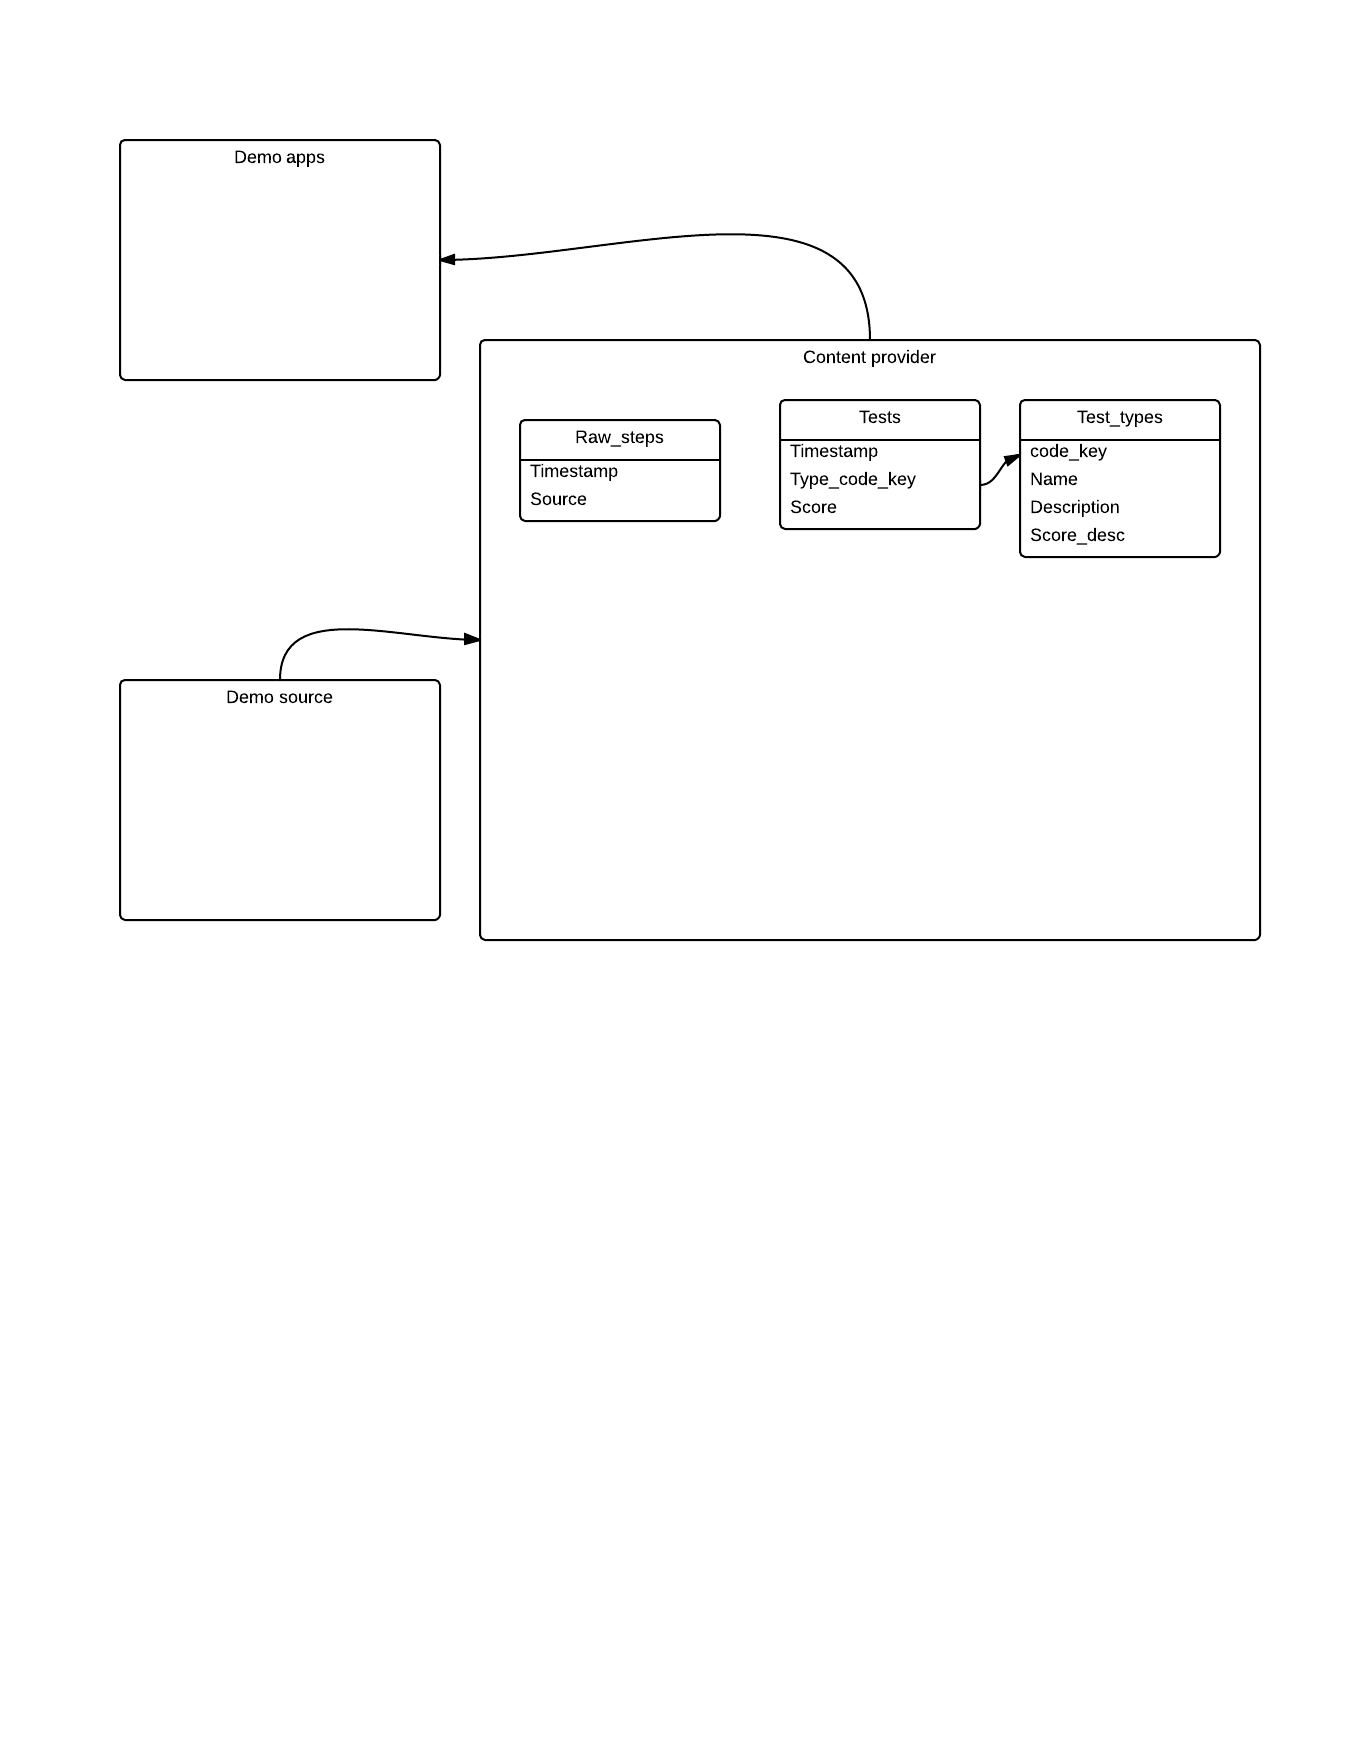
\includegraphics[width=\textwidth, angle = 0]{Res/DataModelContentProvider}
}

\end{figure}